%-----------------------------------------------------------------------
%
%   UFRJ  - Universidade Federal do Rio de Janeiro
%   COPPE - Coordena��o dos Programas de P�s-gradua��o em Engenharia
%   PEE   - Programa de Engenharia El�trica
%
%
%   Projeto ROSA - Rob� para opera��o de stoplogs alagados
%
%   Relat�rio quadrimestral #1
%   Per�odo: Out/2013 a Fev/2014
%
%                                                        20/mar/14, Rio
%                                                        Ramon R. Costa
%----------------------------------------------------------------------
\documentclass[a4paper,11pt,oneside,openany,brazilian,version=last,draft=false]{article}
\usepackage{../macros/mybook}
\usepackage{amsmath,amssymb}  %pacotes do AMS
%\usepackage[latin1]{inputenc} %pacote para entender palavras acentuadas
\usepackage{latexsym}         %pacote para incluir simbolos (ex.\Box)
\usepackage{fancybox,fancyhdr}%pacote com frescuras
\usepackage{graphicx}         %pacote para incluir figuras tipo eps
\usepackage{xcolor}
\usepackage{xspace}
\usepackage{pst-all,pst-poly}  %PSTricks
\usepackage{psfrag}
\usepackage{calc}
\usepackage{multicol}
%\usepackage[english]{babel}
\usepackage{float}
\usepackage{pdfpages}
\usepackage{pdflscape}
\usepackage{geometry}

%----------------------------------------------------------------------
%
%   Macros utilizados no LATEX.
%                                                       Ramon R. Costa
%                                                       23/jun/94, Rio
%----------------------------------------------------------------------
\newcount\m
\newcount\n

\def\twodigits#1{\ifnum #1<10 0\fi \number#1}

\def\hours{\n=\time \divide\n 60
    \m=-\n \multiply\m 60 \advance\m \time
    \twodigits\n:\twodigits\m}

\def\hora{\hours}

\def\data{Rio de Janeiro,\  \number\day\  de \ifcase\month\or
    janeiro\or
    fevereiro\or
    mar\c{c}o\or
    abril\or
    maio\or
    junho\or
    julho\or
    agosto\or
    setembro\or
    outubro\or
    novembro\or
    dezembro\or\fi\  de \number\year}

%----------------------------------------------------------------------

\newcommand{\bl}{\begin{itemize}}           %item point
\newcommand{\el}{\end{itemize}}

\newcommand{\blista}{
    \vspace{-1.5ex}
    \begin{itemize}
    \renewcommand{\labelitemi}{$\Box$}
    \setlength {\itemsep}{-0.8mm}
    \setlength {\parsep} {0mm}
    }

\newcommand{\elista}{
    \end{itemize}
    \vspace{-1ex}
    }

\newcommand{\bd}{\begin{description}}       %item simples
\newcommand{\ed}{\end{description}}

\newcommand{\bn}{\begin{enumerate}}     %item numero
\newcommand{\en}{\end{enumerate}}

\newcommand{\figps}[4]{
    \begin{figure}[htb]
    \centerline{
    \psfig{figure = #4, height = #1cm}
    }
    \caption{#2}
    \label{#3}
    \end{figure}
    }

\newcommand{\mfig}[5]{
    \begin{figure}[htb]
    \centerline{
    \psfig{figure=#5, height=#1cm, width=#2cm}
    }
    \caption{#3}
    \label{#4}
    \end{figure}
    }

\newcommand{\bvect}{\left(\begin{array}{c} }

\newcommand{\evect}{\end{array}\right)}

\newcommand{\mat}[1]{
    \left[
    \begin{array}   % \mat{{cclr} 1&2&3&4 \\ 1&1&1&1}
        #1
    \end{array}
    \right]
}

\newcommand{\matriz}[1]{    %Latex 2e + amstex
    \begin{bmatrix}
        #1
    \end{bmatrix}
}

\newcommand{\equ}[2]{                      % \equ{equation}{label}
  \begin{equation}\label{#2}
  #1
  \end{equation}
}

\newcommand{\dequ}[3]{
    \addtolength{\arraycolsep}{-1mm}
    \renewcommand{\arraystretch}{1.4}
    \begin{equation}
        \begin{array}{rcl}
            #1 \nonumber \\
            #2 \nonumber
        \end{array}
        \label{#3}
    \end{equation}
    \renewcommand{\arraystretch}{1}
    \addtolength{\arraycolsep}{1mm}
}

\newcommand{\tequ}[4]{
    \addtolength{\arraycolsep}{-1mm}
    \renewcommand{\arraystretch}{1.4}
    \begin{equation}
        \begin{array}{rcl}
            #1 \nonumber \\
            #2 \nonumber \\
            #3 \nonumber
        \end{array}
        \label{#4}
    \end{equation}
    \renewcommand{\arraystretch}{1}
    \addtolength{\arraycolsep}{1mm}
}

\newcommand{\cequ}[4]{
    %\addtolength{\arraycolsep}{-1mm}
    \renewcommand{\arraystretch}{1.4}
    \begin{equation}
        #1 = \left\{
        \begin{array}{lcl}
            #2  \\
            #3
        \end{array}
        \right.
        \label{#4}
    \end{equation}
    \renewcommand{\arraystretch}{1}
    %\addtolength{\arraycolsep}{1mm}
}

\newcommand{\eqn}[1]{                      % \equ{equation}{nolabel}
        \begin{equation}
        #1
        \end{equation}
}

\newcommand{\espacoduplo}{\setlength{\baselineskip}{1.5\baselineskip}}
\newcommand{\espacosimples}{\setlength{\baselineskip}{.7\baselineskip}}

\newcommand{\mref}[1]{(\ref{#1})}

%----------------------------------------------------------------------
%
% Agregado por Fernando.
%

\newcommand{\cents}{\hbox{\rm\rlap/c}}
\newcommand{\abs}[1] {\left|#1\right|}
\newcommand{\norm}[1] {\left|\!\left|#1\right|\!\right|}
\newcommand{\vvert}{\Vert}       %always translated to \left| or \right|

%\newcount\notenumber
%\newcommand {\clearnotenumber}{\notenumber=0}
% \newcommand {\note}{\global\advance\notenumber by 1
% \footnote{$^{\the\notenumber}$}}
%\clearnotenumber
%\indice{variavel}{indice}

\newcommand{\indice}[2]{
    #1_{\scriptscriptstyle #2}
}

\newcommand{\espfig}[3]{
        \begin{figure}[htb]
        \vspace{#1cm}
        \caption{{#2}}
        \label{#3}
        \end{figure}
}

\newcommand{\mkfig}[5]{
    \begin{figure}[htb]
        \centerline{
            \psfig{figure=#1.ps,height=#2cm,width=#3cm}
        }
        \caption{{#4}}
        \label{#5}
    \end{figure}
}

%derivee partielle (attention se mettre en mode math)
\newcommand{\dpar}[2]{
    {\frac {\partial #1}{\partial #2}}
}

%derivee partielle (attention se mettre en mode math)
\newcommand{\dnpar}[3]{
    {\frac {\partial ^{#3}#1}{\partial #2^{#3}}}
}

%derivee normale (etre en mode math)
\newcommand{\deriv}[2]{
    {\frac {d #1}{d #2}}
}

\newcommand{\derivn}[2]{
    {\frac {d^{#2}#1}{dt^{#2}}}
}

%----------------------------------------------------------------------
%
% Agregado por Ramon.
%

\newcommand{\CAO}{\c{C}\~{A}O}
\newcommand{\cao}{\c{c}\~{a}o}

\newcommand{\COES}{\c{C}\~{O}ES}
\newcommand{\coes}{\c{c}\~{o}es}

\newcommand{\pee}{Programa de Engenharia El\a'etrica}
\newcommand{\PEE}{PROGRAMA DE ENGENHARIA EL\a'ETRICA}

\newcommand{\coppe}{Coordena\cao\ dos Programas de P\a'os--Gradua\cao\ em Engenharia}
\newcommand{\COPPE}{COORDENA\CAO\ DOS PROGRAMAS DE P\a'OS--GRADUA\CAO\ EM ENGENHARIA}

\newcommand{\ct}{Centro de Tecnologia}
\newcommand{\CT}{CENTRO DE TECNOLOGIA}

\newcommand{\ufrj}{Universidade Federal do Rio de Janeiro}
\newcommand{\UFRJ}{UNIVERSIDADE FEDERAL DO RIO DE JANEIRO}

\newcommand{\rrc}{Ramon Romankevicius Costa}
\newcommand{\RRC}{RAMON ROMANKEVICIUS COSTA}

\newcommand{\ceq}{Comiss\~ao de Exame de Qualifica\cao}
\newcommand{\CEQ}{COMISS\~AO DE EXAME DE QUALIFICA\CAO}

\newcommand{\gscar}{Gru\-po de Si\-mu\-la\-\cao\ e Con\-tro\-le em
            Auto\-ma\-\cao\ e Ro\-b\a'o\-ti\-ca}
\newcommand{\GSCAR}{GRUPO DE SIMULA\CAO\ E CONTROLE EM AUTOMA\CAO\ e ROB\a'OTICA}

\newcommand{\rov}{Ro\-b\^o Sub\-ma\-ri\-no de Ope\-ra\-\cao\ Re\-mo\-ta}
\newcommand{\ROV}{ROB\^O SUBMARINO DE OPERA\CAO\ REMOTA}

\newcommand{\ramon}{
  \vspace{1.5cm}
  \hfill
  \parbox{8cm}{
    \centering
    \rule[0mm]{6cm}{0.1mm} \\[3mm]
    Ramon Romankevicius Costa \\
  }
}

\newcommand{\chefe}{
    \vspace{1.5cm}
    \hspace{7cm}
    \parbox{7cm}{
    \begin{center}
        \rule[0mm]{6cm}{0.1mm} \\
        \vspace{3mm}
        \rrc\\
        \vspace{3mm}
        Chefe da \a'Area de Controle \\
        \pee
    \end{center}}}

\newcommand{\vice}{
    \vspace{1.5cm}
    \hspace{7cm}
    \parbox{7cm}{
    \begin{center}
        \rule[0mm]{6cm}{0.1mm} \\
        \vspace{3mm}
        \rrc\\
        \vspace{3mm}
        Vice--Coordenador \\
        \pee
    \end{center}}}

\newcommand{\coordenador}{
    \vspace{1.5cm}
    \hspace{7cm}
    \parbox{7cm}{
    \begin{center}
        \rule[0mm]{6cm}{0.1mm} \\
        \vspace{3mm}
        \rrc\\
        \vspace{3mm}
        Coordenador \\
        \pee
    \end{center}}}

\newcommand{\orientador}{
    \vspace{1.5cm}
    \hspace{7cm}
    \parbox{7cm}{
    \begin{center}
        \rule[0mm]{6cm}{0.1mm} \\
        \vspace{3mm}
        \rrc\\
        \vspace{3mm}
        Orientador
    \end{center}}}

\newcommand{\liu}{
    \vspace{1.5cm}
    \hfill
    \parbox{8cm}{
    \begin{center}
        \rule[0mm]{6cm}{0.1mm} \\
        \vspace{3mm}
        Liu Hsu \\
%        \vspace{3mm}
%        Chefe do Laborat\'orio de Controle \\
%        \pee
    \end{center}}}

\newcommand{\xEndereco}{
    \vfill
    \begin{small}
    \begin{tabbing}
    Endere\c{c}o :\ \ \= \rrc \\
        \> COPPE/UFRJ --- \pee \\
        \> Caixa Postal 68504 --- CEP 21945--970 --- Rio de Janeiro --- RJ \\
        \> e-mail: {\tt ramon@coep.ufrj.br} \qquad       Fax: 290-6626
    \end{tabbing}
    \end{small}}

\newcommand{\meuendereco}{
    \vfill
    \noindent\rule[0mm]{\textwidth}{0.1mm}
    {\scriptsize \sf
    \begin{minipage}{1.5cm}
        Endere�o :
    \end{minipage}
    \begin{minipage}[t]{8.5cm}
        \rrc\\
        COPPE/UFRJ --- \pee\\
        Caixa Postal 68504 --- CEP 21945--970 --- Rio de Janeiro --- RJ
    \end{minipage}
    \hfill
    \begin{minipage}[t]{4cm}
        \begin{tabbing}
        e-mail\ \= : {\tt ramon@coep.ufrj.br}\\
        Fone    \> : 260-5010 r.267\\
        Fax     \> : 290-6626
        \end{tabbing}
    \end{minipage}
    }}

\newcommand{\laranjeiras}{
    \vfill
    \noindent\rule[0mm]{\textwidth}{0.1mm}
    {\scriptsize \sf
    \begin{minipage}{1.5cm}
        Endere�o :
    \end{minipage}
    \begin{minipage}[t]{8.5cm}
        \rrc\\
        Rua das Laranjeiras, 192/201 \\
        Laranjeiras, CEP 22240--001 --- Rio de Janeiro --- RJ
    \end{minipage}
    \hfill
    \begin{minipage}[t]{4cm}
        \begin{tabbing}
        e-mail\ \= : {\tt ramon@coep.ufrj.br}\\
        Fone    \> : 2265-5520
        Cel.    \> : 9355-8056
        \end{tabbing}
    \end{minipage}
    }}

\newcommand{\Liuendereco}{
    \vfill
    \noindent\rule[0mm]{16.5cm}{0.1mm}
    {\scriptsize \sf
    \begin{minipage}{1.5cm}
        Endere\c{c}o :
    \end{minipage}
    \begin{minipage}[t]{8.5cm}
        Liu Hsu\\
        COPPE/UFRJ --- \pee\\
        Caixa Postal 68504 --- CEP 21945--970 --- Rio de Janeiro --- RJ
    \end{minipage}
    \hfill
    \begin{minipage}[t]{4cm}
        \begin{tabbing}
        e-mail\ \= : {\tt liu@coep.ufrj.br}\\
        Fax     \> : 290-6626
        \end{tabbing}
    \end{minipage}
    }}

\newcommand{\address}{
    \vfill
    \noindent\rule[0mm]{16.5cm}{0.1mm}
    {\scriptsize \sf
    \begin{minipage}{2.3cm}
        Mailing address :
    \end{minipage}
    \begin{minipage}[t]{8.5cm}
        \rrc\\
        COPPE/UFRJ --- Department of Electrical Engineering \\
        P.O. Box 68504 --- 21945--970 --- Rio de Janeiro --- BRAZIL
    \end{minipage}
    \hfill
    \begin{minipage}[t]{4cm}
        \begin{tabbing}
        e-mail\ \= : {\tt ramon@coep.ufrj.br}\\
        Fax     \> : 055 21 290-6626
        \end{tabbing}
    \end{minipage}
    }}

\newcommand{\liuaddress}{
    \vfill
    \noindent\rule[0mm]{16.5cm}{0.1mm}
    {\scriptsize \sf
    \begin{minipage}{2.3cm}
        Mailing address :
    \end{minipage}
    \begin{minipage}[t]{8.5cm}
        Liu Hsu \\
        COPPE/UFRJ --- Department of Electrical Engineering \\
        P.O. Box 68504 --- 21945--970 --- Rio de Janeiro --- BRAZIL
    \end{minipage}
    \hfill
    \begin{minipage}[t]{4cm}
        \begin{tabbing}
        e-mail\ \= : {\tt liu@coep.ufrj.br}\\
        Fax     \> : 290-6626
        \end{tabbing}
    \end{minipage}
    }}

\newcommand{\remetente}{
    \vspace{3cm}
    \parbox{15cm}{
        \rrc \\
        COPPE/UFRJ --- \pee \\
        Caixa Postal 68.504 --- CEP 21.945--970 --- Rio de Janeiro --- RJ
    }
}

\newcommand{\deliver}{
    \vspace{3cm}
    \parbox{15cm}{
        \rrc \\
        COPPE/UFRJ --- Department of Electrical Engineering \\
        P. O. Box 68504 --- 21945--970 --- Rio de Janeiro --- BRAZIL
    }
}

\newcommand{\astrom}{{\AA }str\"{o}m}
\newcommand{\AeW}{\astrom\ \& Wittenmark}
\newcommand{\AeH}{\astrom\ \& H\"agglund}

\newcommand{\fim}{
    \medskip
    \begin{center}
    \rule[1mm]{30mm}{0.14mm}$\diamond$\rule[1mm]{30mm}{0.14mm}
    \end{center}}

\newcommand{\DO}[1]{
    \noindent
    \makebox[8mm][l]{\bf Do }: \parbox[t]{15cm}{#1}

    \smallskip}

\newcommand{\AO}[1]{
    \noindent
    \makebox[8mm][l]{\bf Ao }: \parbox[t]{15cm}{#1}

    }

\newcommand{\AOS}[1]{
    \noindent
    \makebox[8mm][l]{\bf Aos}: \parbox[t]{15cm}{#1}

    }

\newcommand{\A}[1]{
    \noindent
    \makebox[8mm][l]{\bf \`A }: \parbox[t]{15cm}{#1}

    }

\newcommand{\ASSUNTO}[1]{
    \vspace{8mm}
    \noindent
    \hfill {\bf Ref.:} {#1}

    \vspace{5mm}
    }

\newcommand{\diretor}{
    \vspace{1.5cm}
    \hspace{7cm}
    \parbox{7cm}{
    \begin{center}
        \rule[0mm]{6cm}{0.1mm} \\
        \vspace{3mm}
        Prof. Luiz Pinguelli Rosa \\
        \vspace{3mm}
        Diretor da COPPE
    \end{center}}}

%----------------------------------------------------------------------

%----------------------------------------------------------------------
%
%
%     A4 paper size & margins
%
%                                                         Ramon R Costa
%                                                         aug/06/00, SB
%----------------------------------------------------------------------

\setlength {\textheight}    {25cm}%
\setlength {\textwidth}     {17.5cm}%
\setlength {\parindent}     {0mm}%
\setlength {\parskip}       {1mm}%
\setlength {\topmargin}     {-14mm}%
\setlength {\oddsidemargin} {-6mm}%
\setlength {\evensidemargin}{-6mm}%
\setlength {\columnsep}     {6mm}%

%----------------------------------------------------------------------


%-----------------------------------------------------------------------
%
%   UFRJ  - Universidade Federal do Rio de Janeiro
%   COPPE - Coordena��o dos Programas de P�s-gradua��o em Engenharia
%   PEE   - Programa de Engenharia El�trica
%
%
%   Projeto ROSA - Rob� para opera��o de stoplogs alagados
%
%   Macros
%                                                         Ramon R. Costa
%                                                         20/mar/14, Rio
%-----------------------------------------------------------------------
\setlength {\textheight}    {25cm}%
\setlength {\textwidth}     {16.5cm}%{17.5cm}%
\setlength {\parindent}     {5mm}%{0mm}%
\setlength {\parskip}       {3mm}%{1mm}%
\setlength {\topmargin}     {-14mm}%
\setlength {\oddsidemargin} {0mm}%
\setlength {\evensidemargin}{0mm}%
\setlength {\columnsep}     {6mm}%

\newfont{\grande}{cmss10 scaled 1500}
\newfont{\Grande}{cmss10 scaled 2500}
\newfont{\GRANDE}{cmss10 scaled 3500}
\newfont{\enorme}{cmdunh10 scaled 6000}

\newcommand{\BLU}[1]{\colorbox{white}{\textcolor{blue}{#1}}}
\newcommand{\HI}[1]{\colorbox{yellow}{\textcolor{black}{#1}}}  %% Highlithed text

\def\ROSA{\BLU{\textsc{ROSA}}\xspace}
\def\PATH{file:c:/Users/Ramon/My Documents/projetos/2013/Projeto ROSA}

\newcommand{\block}[2]{
  \def\TXT{~#1~}
  \noindent\TXT \hfill
  \parbox[t]{ \textwidth - \widthof{\TXT} - 2mm}{#2} \\
}

\newcommand{\participantes}[1]{
  \block{\textbf{Participantes}:}{#1}
  \medskip%
}

\newcommand{\pauta}[1]{
  \block{\textbf{Pauta}:}{#1}
  \medskip%
}

\newcommand{\dado}[2]{
  \noindent%
  \makebox[30mm][l]{\large\sf#1 {\small\dotfill}} :
  \hfill\parbox[t]{140mm}{#2} %\\[2mm]
  \par
  \vspace*{0.30mm}
}

\newcommand{\vu}[2]{ %Utiliza��o: \vu{valor}{unidade}
  \textcolor{darkblue}{#1$\,#2$}\xspace
}

\def\alana{Alana Monteiro\xspace}
\def\antonio{Ant�nio\xspace}
\def\jacoud{Alessandro Jacoud\xspace}
\def\andre{Andr� Figueir�\xspace}
\def\breno{Breno Bellinati de Carvalho\xspace}
\def\elael{Eduardo Elael\xspace}
\def\gabriel{Gabriel Alc�ntara\xspace}
\def\gizele{Gizele Ferreira da Silva\xspace}
\def\julia{J�lia Campana\xspace}
\def\patrick{Patrick Paranhos\xspace}
\def\rafael{Rafael Oliveira\xspace}
\def\ramonC{Ramon Campos\xspace}
\def\ramon{Ramon Romankevicius\xspace}
\def\renan{Renan Freitas\xspace}
\def\sylvain{Sylvain Joyeux\xspace}



\begin{document}
%---------------------------------------------------------------------
\pagestyle{fancy}%
\thispagestyle{fancy}%
\renewcommand{\headrulewidth}  {0.4pt}%
\renewcommand{\footrulewidth}  {0.4pt}%
\lhead{\vspace*{-5mm}
\includegraphics[width=30mm]{../logo/lead-logo.jpg}}%
\chead{}%
\rhead{}%
\lfoot{}%
\cfoot{}%
\rfoot{\today}%
%---------------------------------------------------------------------
\vspace*{20mm}%

{\grande \textcolor{gray}{Financiamento}}

\vspace{-15mm}%
\hspace{50mm}%

\includegraphics[width=50mm]{../logo/esbr-logo.png}
\hspace{10mm}%

\includegraphics[width=40mm]{../logo/aneel-logo.jpg}

\vspace{35mm}%
{\grande \textcolor{gray}{Execu��o}}

\vspace{-25mm}%
\hspace{50mm}%

\includegraphics[width=50mm]{../logo/gscar-logo.png}
\hspace{10mm}%

\includegraphics[width=40mm]{../logo/coppetec50-logo.jpg}

\vfill%
\begin{center}
  {\GRANDE \raisebox{1.4ex}{\textcolor{gray}{Projeto}} 
\includegraphics[width=70mm]{../logo/logo_land_ROSA.jpg}} \\[10mm]
  {\Grande Rob� para opera��o de stoplogs alagados} \\[25mm]
  {\Grande Relat�rio quadrimestral \#1} \\[5mm]
  {\Grande Per�odo: Out/2013 a Fev/2014} \\
  \vfill%
  %{\Large Fevereiro de 2014} \\[8mm]
\end{center}

\newpage%
%---------------------------------------------------------------------
\pagestyle{fancy}%
\renewcommand{\headrulewidth}  {0.4pt}
\renewcommand{\footrulewidth}  {0.4pt}
\lhead{\vspace*{-6mm}
\includegraphics[width=30mm]{../logo/lead-logo.jpg}}%
\chead{\vspace*{-6mm}\raisebox{1.7ex}{\textcolor{gray}{Projeto}} 
\includegraphics[width=30mm]{../logo/logo_land_ROSA.jpg}}%
\rhead{\sf\thepage}%
\lfoot{Relat�rio quadrimestral \#1}%
\cfoot{}%
\rfoot{\sf [\hours] \quad \today}%
%---------------------------------------------------------------------

\tableofcontents

\newpage%
%---------------------------------------------------------------------
\section{Identifica��o}

%-----------------------------------------------------------------------
%
%   UFRJ  - Universidade Federal do Rio de Janeiro
%   COPPE - Coordena��o dos Programas de P�s-gradua��o em Engenharia
%   PEE   - Programa de Engenharia El�trica
%
%
%   Projeto ROSA - Rob� para opera��o de stoplogs alagados
%
%   Identifica��o
%                                                         Ramon R. Costa
%                                                         20/mar/14, Rio
%-----------------------------------------------------------------------
%\section{Identifica��o}

\dado{T�tulo}{
  ROSA - Rob� para opera��o de \emph{stoplogs} alagados \\
}

\dado{Proponente}{
  Universidade Federal do Rio de Janeiro (UFRJ) \\[2mm]
  Funda��o Coordena��o de Projetos, Pesquisas e Estudos Tecnol�gicos (COPPETEC) \\
}

\dado{Contratante}{
  Energia Sustent�vel do Brasil S.A. \\
}

\dado{Execu��o}{
  Grupo de Simula��o e Controle em Automa��o e Rob�tica (GSCAR) \\
}

\dado{Contrato}{
  Jirau 151/13 \\
}

\dado{P\&D ANEEL}{
  6631-0002/2013 \\
}

\dado{COPPETEC}{
  PEE 17.369 \\
}

\dado{In�cio}{
  08 de Outubro de 2013 \\
}

\dado{Prazo}{
  12 meses \\
}

\dado{Or�amento}{
  R\$ 4.364.217,78 \\
}

\dado{Coordenador}{
  Ramon Romankevicius Costa \\
}

\dado{Gerente}{
  Breno Bellinati de Carvalho \\
}

%---------------------------------------------------------------------
\fim


\newpage%
%---------------------------------------------------------------------
\section{Equipe executora}

%-----------------------------------------------------------------------
%
%   UFRJ  - Universidade Federal do Rio de Janeiro
%   COPPE - Coordena��o dos Programas de P�s-gradua��o em Engenharia
%   PEE   - Programa de Engenharia El�trica
%
%
%   Projeto ROSA - Rob� para opera��o de stoplogs alagados
%
%   Identifica��o
%                                                         Ramon R. Costa
%                                                         20/mar/14, Rio
%-----------------------------------------------------------------------
%\section{Equipe}

\renewcommand{\arraystretch}{1.4}
\begin{center}
\begin{small}
\begin{tabular}{|l|l|c|c|l|}
\hline
\makebox[45mm][c]{\bf Nome} &
    \makebox[25mm][c]{\bf Fun��o} &
    \makebox[25mm][c]{\bf Qualifica��o} &
    \makebox[25mm][c]{\bf Institui��o} &
    \makebox[25mm][c]{\bf CPF} \\
\hline
\hline
  \alana   & Auxiliar Adm. & SU & UFRJ & 147.881.217-60 \\
  \jacoud  & Pesquisador   & DO & UFRJ & 028.503.687-41 \\
  \andre   & Pesquisador   & SU & UFRJ & 124.207.057-05 \\
  \elael   & Pesquisador   & SU & UFRJ & 045.287.677-08 \\
  \gabriel & Pesquisador   & SU & UFRJ & 136.759.937-79 \\
  \julia   & Pesquisador   & SU & UFRJ & 102.517.697-98 \\
  \patrick & Pesquisador   & MS & CIR  & 092.144.157-65 \\
  \ramon   & Coordenador   & DO & UFRJ & 310.036.646-87 \\
  \renan   & Pesquisador   & SU & UFRJ & 129.325.817-24 \\
%  \breno   & Gerente       & SU & ESBR & 0000000 \\
%  \gizele  & Auxiliar Adm. & SU & ESBR & 0000000 \\
\hline
\end{tabular}
\end{small}
\end{center}
\renewcommand{\arraystretch}{1}

%---------------------------------------------------------------------
\fim


%---------------------------------------------------------------------

%%******************************************************************************
%% SECTION - Cronograma
%%******************************************************************************
\section{Cronograma}
\label{cronograma}

%\vspace{-5mm}%
\begin{center}
    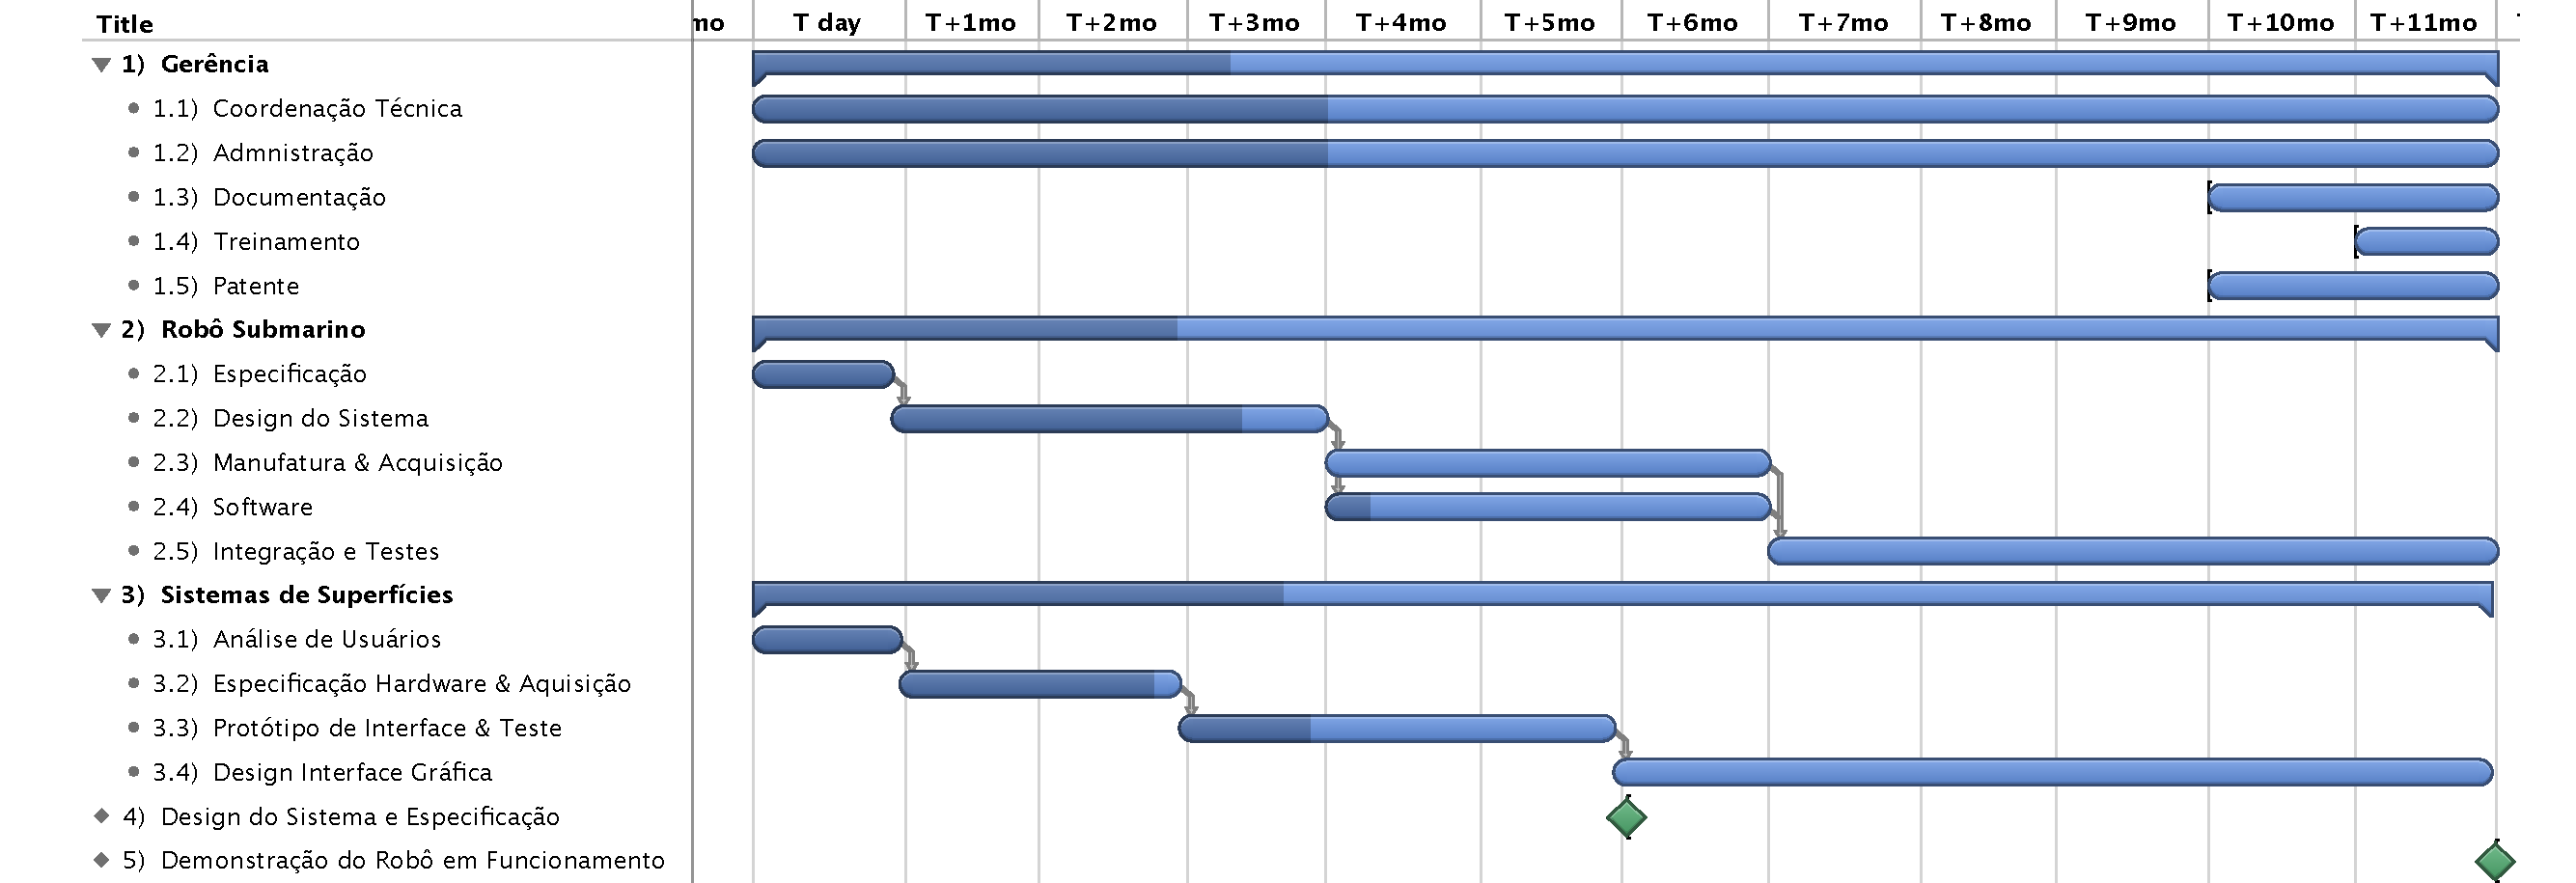
\includegraphics[angle=90,scale=0.55]{figs/gantt/Gantt.pdf}
\end{center}

\newpage%
{\bf  1) Ger�ncia}: Planejamento tecnol�gico e administrativo, organiza��o, coordena��o e controle utilizados para alcan�ar os objetivos gerais do projeto, que n�o estejam associados a hardware espec�fico ou elementos de software.

\begin{description}

\item[1.1) Coordena��o T�cnica:] Coordenar a parte t�cnica do projeto, atribuindo tarefas e revendo o trabalho conclu�do. O resultado da coordena��o t�cnica no per�odo e seus entreg�veis foram:

\begin{description}
	\item [Status] - Tarefa em andamento, sem atrasos.
	\item [Entreg�vel 01] - Atas de reuni�es de acompanhamento t�cnico e aloca��o de tarefas.
	\item [Entreg�vel 02] - Relat�rios Mensais 01, 02 e 03.
	\item [Entreg�vel 03] - Relat�rio Quadrimestral 01.
\end{description}


\item[1.2) Administra��o:]  Administrar a parte financeira do projeto. O resultado s�o as planilhas do balan�o financeiro do projeto atualizadas.

\begin{description}
	\item [Status] - Tarefa em andamento, sem atrasos.
	\item [Entreg�vel 01] - Relat�rio Mensais 01, 02 e 03.
	\item [Entreg�vel 02] - Relat�rio Quadrimestral 01.
\end{description}


	\item[1,3) Documenta��o:] Este pacote de trabalho lida com a escrita da documenta��o t�cnica e de opera��es. Os resultados s�o os manuais e a documenta��o t�cnica do sistema.

\begin{description}
	\item [Status] - Tarefa n�o iniciada.
\end{description}

	\item[1,4) Treinamento:] Esfor�o necess�rio para treinar o pessoal de opera��o da hidrel�tricas no uso do  sistema rob�tico desenvolvido no projeto.

\begin{description}
	\item [Status] - Tarefa n�o iniciada.
\end{description}

	\item[1,5) Patente:] Solicita��o de patente de produto para o sistema rob�tico desenvolvido.

\begin{description}
	\item [Status] - Tarefa n�o iniciada.
\end{description}

\end{description}


\begin{description}

\vspace{0,5cm}

\item[ 2)  Rob� Submarino:] Este elemento lida com o trabalho necess�rio para desenvolver o sistema eletromec�nico do rob�.

\item[2,1) Especifica��o:] neste pacote de trabalho, requisitos do sistema ser�o especificados atrav�s de reuni�es com os funcion�rios respons�veis pela opera��o na hidroel�trica e atrav�s de observa��es em campo. O resultado ser� um documento com os requisitos do sistema.

\begin{description}
	\item [Status] - Tarefa Conclu�da.
	\item [Entreg�vel 01] - Documento de Projeto B�sico.
\end{description}

\item[2,2) Design do Sistema:] Processo de defini��o da arquitetura, componentes, m�dulos e interface que satisfazem os requisitos do sistema. O resultado ser� uma lista de componentes, arquitetura de software e design eletromec�nicos do sistema.

\begin{description}
	\item [Status] - Tarefa em Andamento, atraso de de 1 m�s. A lista de componentes e design el�trico previsto para este pacote de trabalho foram conclu�dos e est�o detalhados no documento de Projeto B�sico. Entretanto, dado os atrasos de pagamento das parcelas do projeto n�o foi poss�vel contratar os servi�os de design mec�nico e de software.
\end{description}

\item[2,3) Manufatura e Aquisi��o:] Compra e constru��o dos componentes definidos durante a fase de design do sistema. O resultado ser�o as partes que integradas formar�o o rob�.

\begin{description}
	\item [Status] - Tarefa n�o iniciada.
\end{description}

\item[2,4) Software:] Desenvolvimento de drivers, controladores e comunica��o para o hardware do rob�. O resultado ser� uma biblioteca de componentes  do software.

\begin{description}
	\item [Status] - Tarefa iniciada.
\end{description}

\item[2,5) Integra��o e Teste:] Os componentes eletr�nicos, mec�nicos e de software ser�o integrado no sistema Viga Pescadora Inteligente. Este pacote de trabalho tamb�m inclui a instala��o e teste do sistema.

\begin{description}
	\item [Status] - Tarefa n�o iniciada.
\end{description}

\end{description}


\begin{description}

\vspace{0,5cm}

\item[3) Sistemas de Superf�cie:] Este elemento inclui o hardware e o software necess�rios para a opera��o do rob� na superf�cie, incluindo a concep��o, desenvolvimento, implementa��o e integra��o da comunica��o, interface e ger�ncia de dados.

\item[3,1) An�lise de Usu�rio:] An�lise dos potenciais usu�rio do sistemas. Este pacote de trabalho vai resultar em um documento que define: O que o usu�rio espera do sistema. Como o sistema ir� fazer parte do dia a dia da opera��o. Qual � a capacita��o t�cnica do futuro usu�rio. Qual apar�ncia de interface t�m um maior apelo para o usu�rio.

\begin{description}
	\item [Status] - Tarefa Conclu�da.
	\item [Entreg�vel 01] - Documento de An�lise de Usu�rio.
\end{description}

\item[3,2) Especifica��o de Hardware e Aquisi��o:] Este pacote de trabalho inclui a especifica��o e aquisi��o do equipamento necess�rio para operar o rob� a partir da superf�cie. O resultado � um lista de componentes e respectivos fabricantes a serem comprados para o projeto.

\begin{description}
	\item [Status] - Tarefa Atrasada, 1 m�s. O equipamento foi especificado entretanto devido ao atraso do pagamento das parcelas do projeto a aquisi��o n�o foi realizada.
\end{description}


\item[3,3) Prot�tipo de Interface e Teste:] Desenvolvimento de telas interativas simples, sem conte�do, concentrando apenas no desenvolvimento da parte visual da interface. Estes prot�tipo de interface vai ser testado com os futuros usu�rio dos sistema e o resultado da sensa��o da mesma ser� avaliada.

\begin{description}
	\item [Status] - Tarefa iniciada.
\end{description}

\item[3,4) Interface de Usu�rio:] Implementa��o da interface de usu�rio (GUI) do rob�, o que permite a visualiza��o e o seu controle. O resultado ser� um software.

\begin{description}
	\item [Status] - Tarefa n�o iniciada.
\end{description}


\end{description} 
%%******************************************************************************
%% SECTION - Financeiro
%%******************************************************************************
%\def\real{R\$}
\def\real{}

\section{Financeiro}
\label{financeiro}
\vfill
\begin{center}
    \begin{tabular}{|c|r|r|r|r||r}
    \hline
		
	{\bf .} &	{\bf Percentual} &	{\bf Estimado }	&	{\bf Despesas}&		{\bf Desembolso}&		{\bf Balan�o}   	\\  \hline

	RH&  13,00 \%& 1.027.409 \real & 	 	137.364,37 \real & 	 	0 \real & 	 	- 137.364,37 \real  \\ \hline

	ST&  0,00 \%& 700.000 \real & 	 	0 \real & 	 	0 \real & 	 	0 \real 	\\  \hline

	MC &  0,00 \%& 2.500 \real& 	 	0 \real& 	 	0 \real  & 	 	0 \real 	\\  \hline	

	MP&  0,00 \%& 1.972.875 \real& 	 	0 \real& 	 	0 \real & 	 	0 \real 	\\  \hline				 

	VD&  0,00 \%& 158.160 \real& 	 	0 \real& 	 	0 \real & 	 	0 \real	\\  \hline

	OU&  0,00 \%& 503.273 \real& 	 	0 \real& 	 	0 \real & 	 	  \real 	 \\  \hline
	\hline
		{\bf Total} 	&  3 \%&  4.364.217,78 \real& 	 	0 \real & 	 0 \real &	-137.364,37 \real 	 \\  \hline

\end{tabular}
\end{center}

\vfill

\begin{center}
  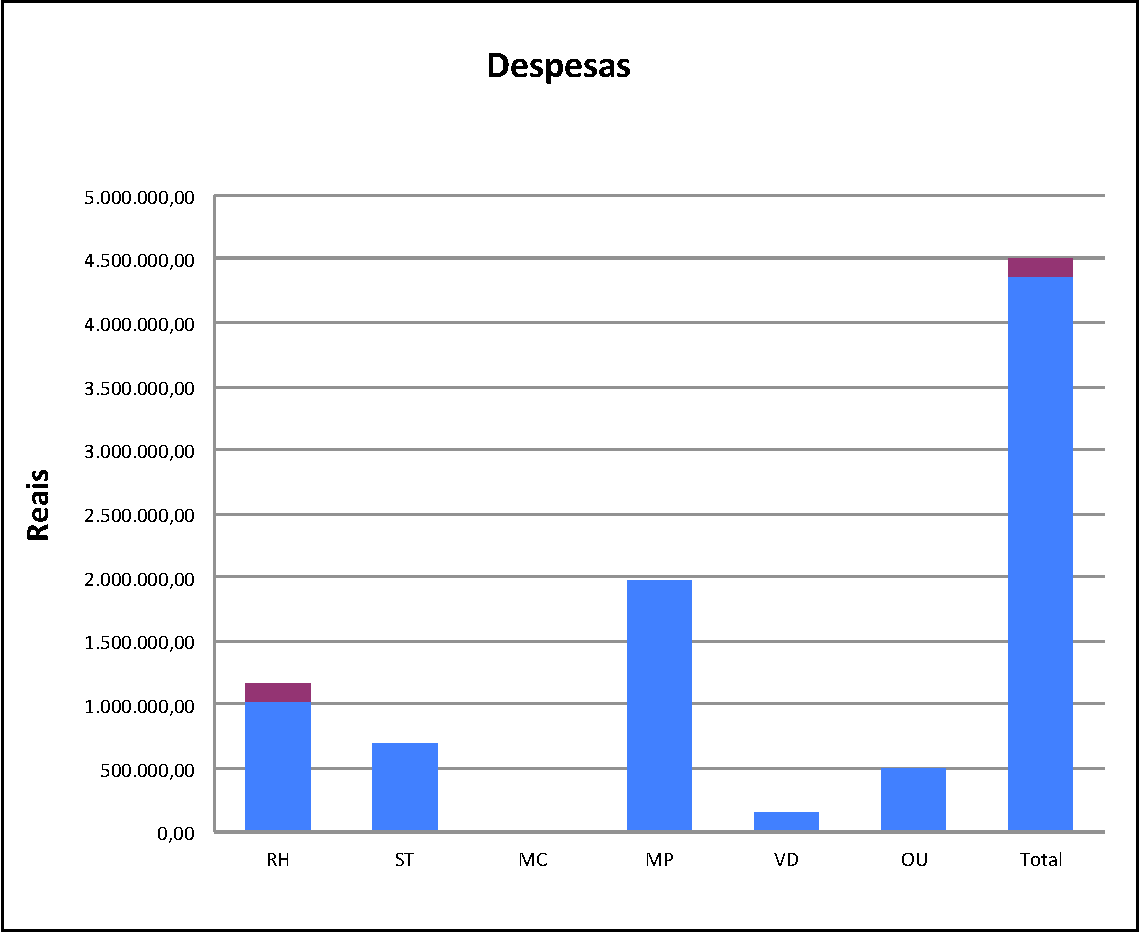
\includegraphics[width=1\columnwidth]{figs/financeiro/financeiro.pdf}
\end{center}


\vfill

\newpage

\subsection{Recursos Humanos}


\begin{center}
  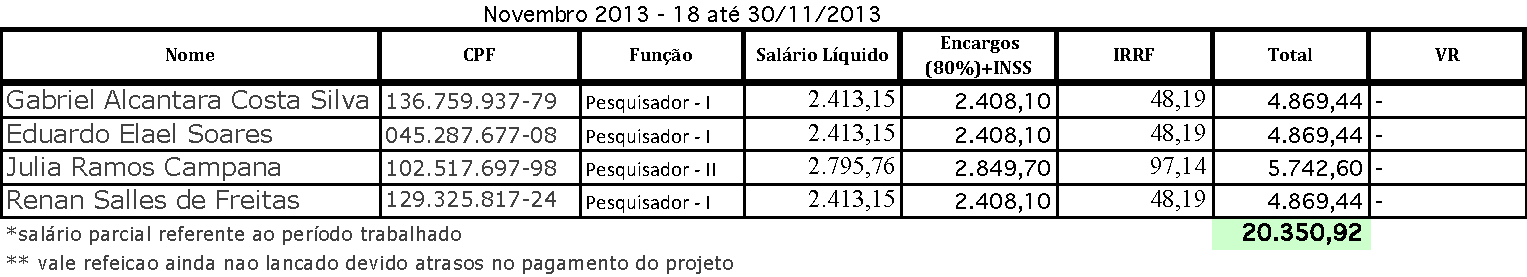
\includegraphics[width=1\columnwidth]{figs/financeiro/RH_novembro.pdf}
\end{center}

\begin{center}
  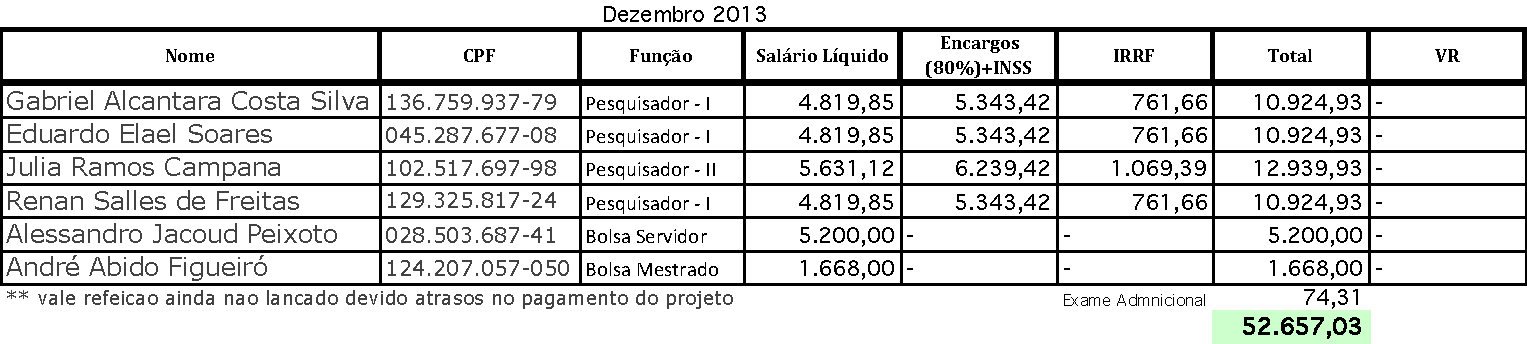
\includegraphics[width=1\columnwidth]{figs/financeiro/RH_dezembro.pdf}
\end{center}

\begin{center}
  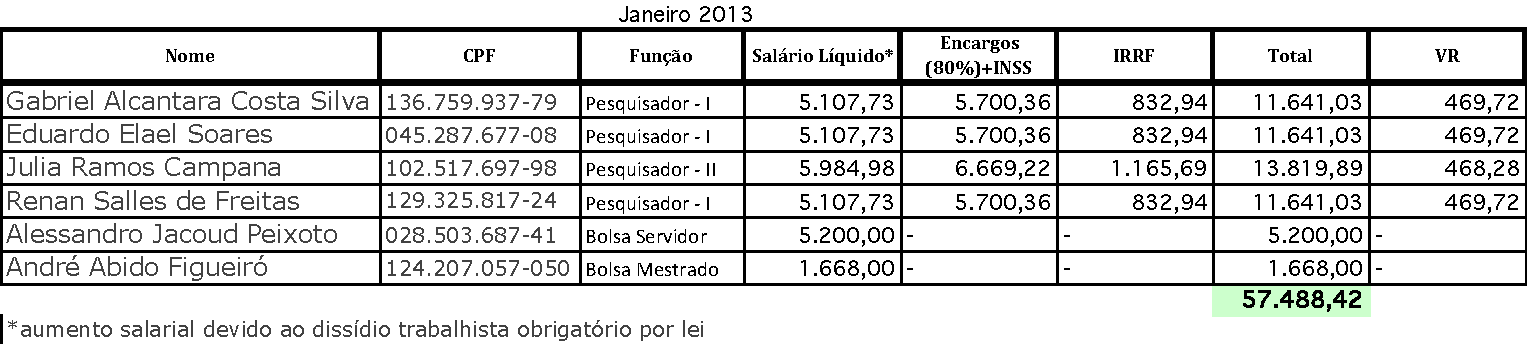
\includegraphics[width=1\columnwidth]{figs/financeiro/RH_janeiro.pdf}
\end{center}

Obs: Os exames admissionais foram executados antes da contrata��o, entretanto s� foram lan�ado no sistema no m�s de dezembro

\subsection{Servi�o de Terceiro}
Nenhum servi�o foi contratado para o projeto.

\subsection{Material de consumo}
Nenhum material de consumo foi comprado para o projeto.

\subsection{Materiais permanentes}
Nenhum material permanente foi comprado para o projeto.

\subsection{Viagens e di�rias}
Nenhuma despesa com viagens e di�rias ocorreu no per�odo.

\subsection{Outros}
Nenhum gasto com outros no per�odo.






%%******************************************************************************
%% SECTION -•	C�lculos e modelagens;
%%******************************************************************************
\setcounter{secnumdepth}{3}
\section{C�lculos e modelagens}
\label{calculos_e_modelagens}

Nenhum c�lculo ou modelo foi desenvolvido no quadrimestre.


%%******************************************************************************
%% SECTION - Resultados alcan�ados (resumo de medidas efetuadas, resultados de an�lises e ensaios, especifica��es de prot�tipos, etc.);
%%******************************************************************************
\setcounter{secnumdepth}{3}
\section{Resultados alcan�ados}
\label{resultados_alcancados}

No primeiro quadrimestre do projeto foi realizado a defini��o do rob� ROSA, seu modo de opera��o e seus componentes. O detalhamento do mesmo e a racionaliza��o pelas escolhas de cada componente se encontra no documento de Projeto B�sico em anexo. Aqui ser� apresentado apenas um resumo do resultado alcan�ado.

O sistema ROSA � composto pelos sensores:
\begin{itemize}
\item Dois encoders absolutos;
\item Dois sensores indutivos de proximidade;
\item Sensor de inclina��o;
\item Sensor de profundidade e
\item Sonar profiling com unidade de Pan \& Tilt.
\end{itemize}

Os encoders ser�o acoplados ao eixo de rota��o da garra pescadora. O
monitoramento do deslocamento angular das garras torna
poss�vel a identifica��o de falhas de encaixe. Durante a opera��o de encaixe, o
eixo da garra percorre �ngulos j� conhecidos. O �ngulo de rota��o sofre leve deslocamento e
retorna � posi��o correspondente ao encaixe.

Os sensores indutivos de proximidade ser�o instalados na garra pescadora,
pr�ximo ao local de contato com o \emph{Stoplog}. O campo magn�tico gerado indicar� o acoplamento das garras
com o \emph{Stoplog}. Esses sensores s� ser�o
excitados em casos de proximidade com metais, sendo poss�vel assim a
identifica��o de obst�culos no encaixe do \emph{Stoplog}.

O sensor de inclina��o ficar� localizado junto � eletr�nica embarcada, na parte
central do Lifting Beam. O monitoramento da inclina��o do Lifting Beam �
importante para a identifica��o de encaixe mal sucedido ou danos no equipamento. O
sensor ser� do tipo capacitivo.

O sensor de profundidade tamb�m ficar� localizado junto � eletr�nica embarcada,
na parte central do Lifting Beam. O sensor trabalha com diferen�a de press�o e
ser� importante na identifica��o da localiza��o do Lifting Beam quando submerso.

O sonar ser� acoplado � unidade Pan e Tilt, sendo o conjunto acoplado � base do lifting beam. Este conjunto ser� utilizado para realizar a inspe��o atrav�s de mapeamento 3D do trilho do \emph{Stoplog} e dos olhais do \emph{Stoplog}.

Estes sensores ser�o conectados a uma eletr�nica embarcada submarina que ir� processar os dados e transmiti-los para a superf�cie atrav�s de um umbilical.

A eletr�nica embarcada � composta por:

\begin{itemize}
	\item PC embarcado industrial com ethernet, RS485 e interface CAN;
	\item Conversores DC/DC;
    \item Placa microcontroladora com sensor de inclina��o, sensor de profundidade, sensor de ingresso de �gua e portas para 2 sensores anal�gicos e
	\item Circuito supervis�rio.
\end{itemize}

A eletr�nica embarcada ter� encapsulamento a prova de  �gua,
choque e resist�ncia m�nima de 5 bar de press�o. O encapsulamento deve possuir 8 conectores Subconn a prova d'�gua para conectar os sensores externos:

\begin{itemize}
 	\item Um Super Seaking Profiler DFP from Tritech;
 	\item Um Gemini 720i from Tritech;
	\item Um Micron Sonar DST 750m from Tritech;
	\item Um OE10-10 from Kongsberg;
	\item Dois NBB20-L2-E2-V1 from Pepperl-Fuchs e
	\item Dois RM9000 from IFM.
\end{itemize}

O circuito supervis�rio ser� respons�vel por distribuir a alimenta��o aos
dispositivos, monitorar essa pot�ncia fornecida e proteger os equipamentos
contra sobrecorrente/voltagem. Ser� composta por rel�s, microcontroladores e
outros componentes eletr�nicos.

Conversores DC/DC realizam o condicionamento do sinal. Os dispositivos t�m
alimenta��o variada e o umbilical fornece apenas um n�vel de tens�o, dessa forma
h� a necessidade de conversores para distribu�rem a pot�ncia como requerida
entre os dispositivos.

A eletr�nica embarcada ser� conectada a uma eletr�nica de terra por um umbilical e operar� submersa.

O Umbilical � um cabo especial  de alta resist�ncia mec�nica para opera��o submersa customizado para transmiss�o de energia e transmiss�o de dados. O umbilical fornece conex�o de dados entre o sistema eletr�nico embarcado e a eletr�nica de terra. Al�m disso, o sistema eletr�nico embarcado � alimentado pelo umbilical. A taxa de transmiss�o m�nima necess�ria para o Umbilical � de 1xRS485

A eletr�nica de superf�cie na base ser� composta por:

\begin{itemize}
	\item PC Industrial com interface Wi-Fi;
	\item 230V de entrada de alimenta��o;
	\item Interfaces USB e LAN para perif�ricos e
	\item Caixa Policase para a eletr�nica.
\end{itemize}

A fonte ir� transmitir a pot�ncia necess�ria a todo o sistema embarcado
atrav�s do umbilical.

O PC processar� todos os dados recebidos do sistema embarcado e publicar� na
internet ou disponibilizar� atrav�s do WiFi.

O operador poder� monitorar todos os sensores atrav�s de um tablet com sistema
de rede WiFi.

Para realizar a ger�ncia do umbilical de maneira aut�noma ser� pesquisado a possibilidade de se instalar um carretel industrial no guindaste. A defini��o do carretel ainda n�o foi conclu�da.





%%******************************************************************************
%% SECTION - Descri��o sum�ria da metodologia adotada no desenvolvimento das etapas;
%%******************************************************************************
\setcounter{secnumdepth}{3}
\section{Metodologia}
\label{metodologia}

Ap�s a an�lise e compreens�o do problema de inser��o e remo��o de \emph{Stoplogs} em visita de campo, foi feita uma
\textbf{Pesquisa Bibliogr�fica} e \emph{brainstorm} com o objetivo de alcan�ar um conceito s�lido de solu��o para o problema.

A partir do resultado dessa pesquisa foi desenvolvido um conceito base de solu��o rob�tica, descrito na se��o {\bf Escopo} do projeto b�sico. Baseado neste conceito, foram realizadas pesquisas de tecnologias e de fornecedores (se��o  {\bf Pesquisa Tecnol�gica} do projeto b�sico) de forma recursiva e convergente com rela��o aos resultados. Isto
�, com base nas pesquisas de solu��o tecnol�gicas poss�veis, buscam-se fornecedores compat�veis e com o
resultado e informa��o dos produtos dos fornecedores encontrados faz-se
novamente uma pesquisa de tecnologia, agora mais aprofundada, e assim sucessivamente
at� encontrar-se um resultado final satisfat�rio.

Esta pesquisa j� � focada nos
componentes a serem utilizados, dessa maneira, os fornecedores escolhidos eram
baseados n�o somente na conformidade t�cnica, mas tamb�m tempo de entrega,
dificuldade de importa��o, suporte e reconhecimento. O escopo inicial de solu��o
� ent�o atualizado e detalhado de acordo com o resultado desta pesquisa, resultando na descri��o do rob� a ser constru�do no projeto.


%%******************************************************************************
%% SECTION - Reuni�es, palestras e cursos realizados (internos e externos);
%%******************************************************************************

\section{Reuni�es, palestras e cursos}
\label{reunioes_palestras_e_cursos}

As reuni�es de acompanhamento t�cnico foram realizadas nas datas relacionadas abaixo (as atas encontram-se em anexo):

\begin{itemize}
	\item 25 de Outubro de 2013;
	\item 1, 6, 11, 18, 25 de Novembro de 2013;
	\item 2, 9, 17 de Dezembro de 2013;
	\item 9, 13, 21, 27 de Janeiro de 2014;
	\item 3, 14, 18, 24 de  Fevereiro de 2014.
\end{itemize}

A reuni�o de abertura do projeto e an�lise do problema foi realizada em Jirau em:

\begin{itemize}
	\item 11 de Novembro de 2013.
\end{itemize}

No dia 18 de Fevereiro de 2014 foi realizada uma reuni�o de alinhamento administrativo entre a ESBR e a COPPETEC.
   	




%%******************************************************************************
%% SECTION - Viagens Realizadas
%%******************************************************************************
\setcounter{secnumdepth}{3}
\section{Viagens}
\label{viagens}

A viagem a Usina Jirau aconteceu entre os dias 10 e 13 de Novembro de 2013. A
equipe visitante foi formada por \patrick, \ramon, \jacoud
e \julia. A viagem teve um car�ter inicial e o objetivo foi realizar a
reuni�o de abertura, passando por  uma an�lise inicial do problema, assim como o acompanhamento de
uma opera��o com \emph{Stoplog}. Complementarmente, a visita proporcionou ao
grupo a oportunidade de conhecer pessoalmente os respons�veis pelo projeto na
ESBR.
Na reuni�o de abertura, esclarecemos quest�es de ordem t�cnica e tamb�m quest�es
ligadas aos procedimentos da ESBR em Projetos de Pesquisa e Desenvolvimento (P$\&$D), assim como foi realizada a assinatura da Ordem de Servi�o do Projeto.  Por parte da ESBR estavam presentes \breno, \ramonC e \gizele. Ap�s a reuni�o de abertura fomos conduzidos a um pequeno ``tour''
pela usina afim de conhecer melhor as instala��es e as atividades l� realizadas.

\begin{figure}[ht!]
    \centering 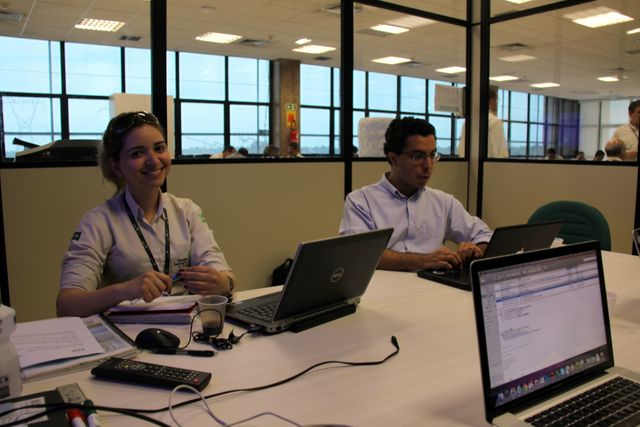
\includegraphics[width=0.6\columnwidth]{figs/jirau/jirau_01}
    \caption{Reuni�o de abertura.}
    \label{fig:jirau1}
\end{figure}



%%******************************************************************************
%% SECTION - Apresentar outras informa��es relevantes. Por exemplo, o recebimento de pr�mios;
%%******************************************************************************

\section{Outros}
\label{outros}

A defini��o do tema de pesquisa do bolsista de mestrado Andr� Figueir� e sua justificativa de alinhamento junto aos objetivos do projeto ROSA foi conclu�da no per�odo. 
\newpage
\appendix
\section{Ap�ndices} \label{App:Appendix}

Seguem em anexo a este relat�rio os seguintes documentos:

\begin{enumerate}
  \item Minutas das reuni�es semanais realizadas neste quadrimestre;
  \item Relat�rio geral \#1 do projeto ROSA e
  \item Proposta de tese de \andre.
\end{enumerate}

\newpage%
\subsection{Ap�ndice 1 - Minutas das reuni�es}
\label{Apendice 1}
%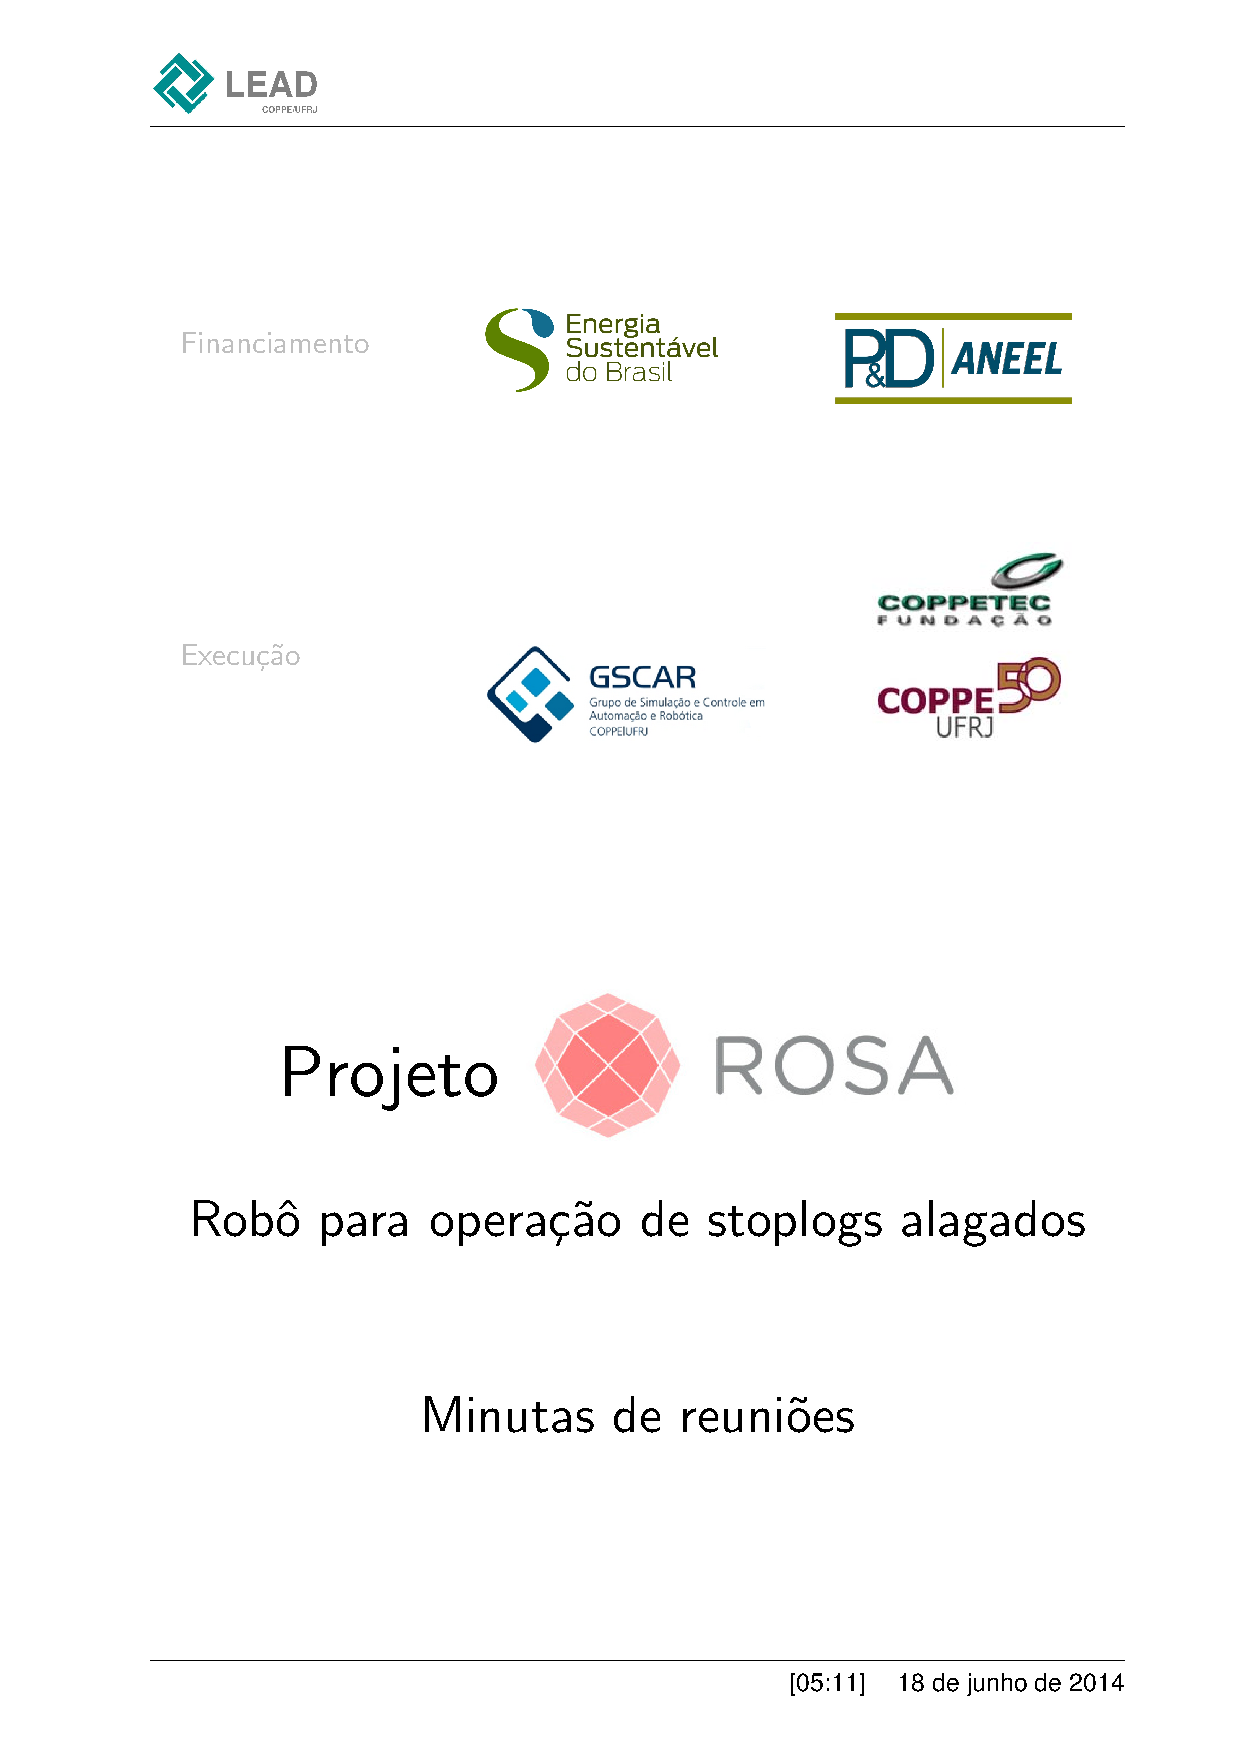
\includepdf[pages=-]{'../minutas (by RRC)/ROSA - minutas de reunioes.pdf'}
%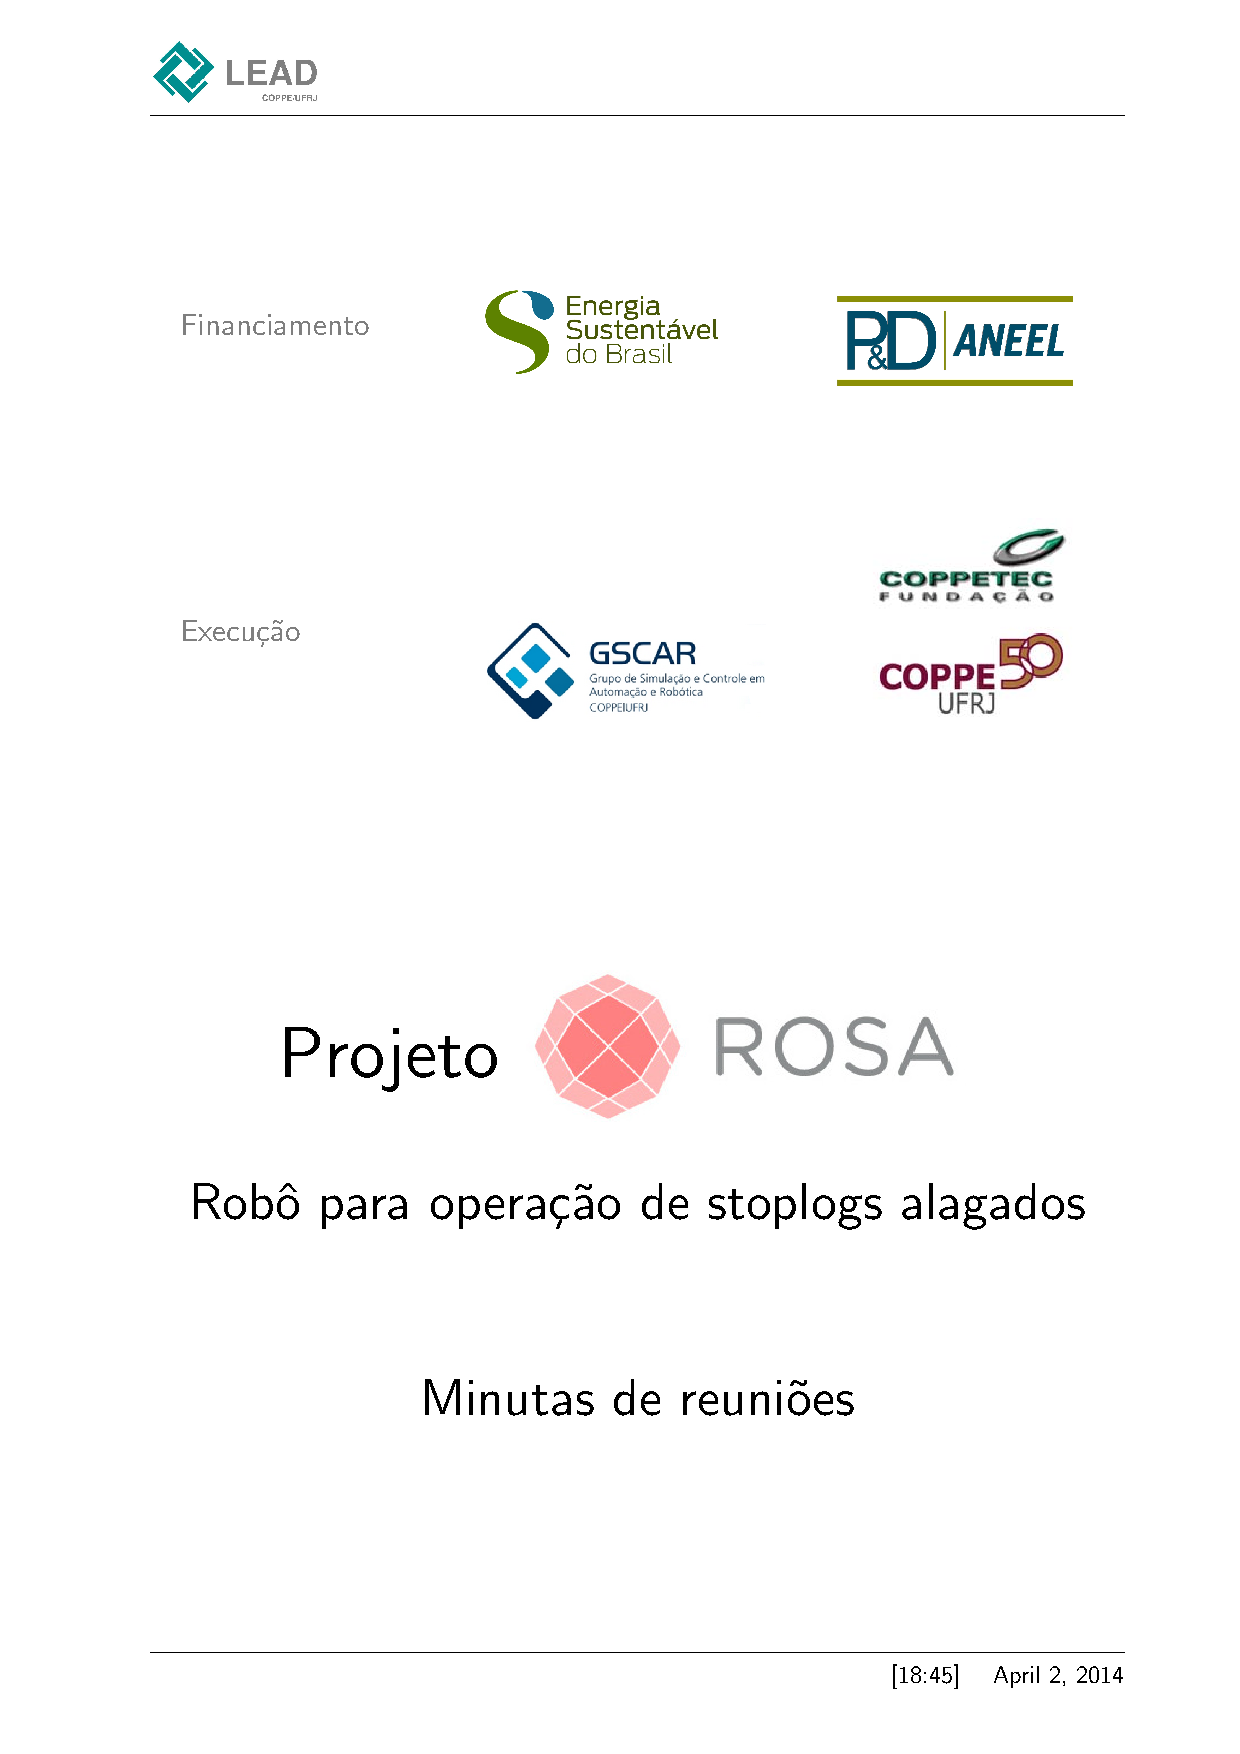
\includepdf[pages=-]{apendice-1-minutas.pdf}

\newpage%
\subsection{Ap�ndice 2 - Relat�rio geral \#1}
\label{Apendice 2}
%\includepdf[pages=-]{'../relatorio geral (by RRC)/ROSA - relatorio geral (fev-2014).pdf'}
%\includepdf[pages=-]{apendice-2-relatorio-geral.pdf}

\newpage%
\subsection{Ap�ndice 3 - Proposta de tese}
\label{Apendice 3}
%\includepdf[pages=-]{../proposta de tese do Andre/proposta de tese do Andre.pdf}
%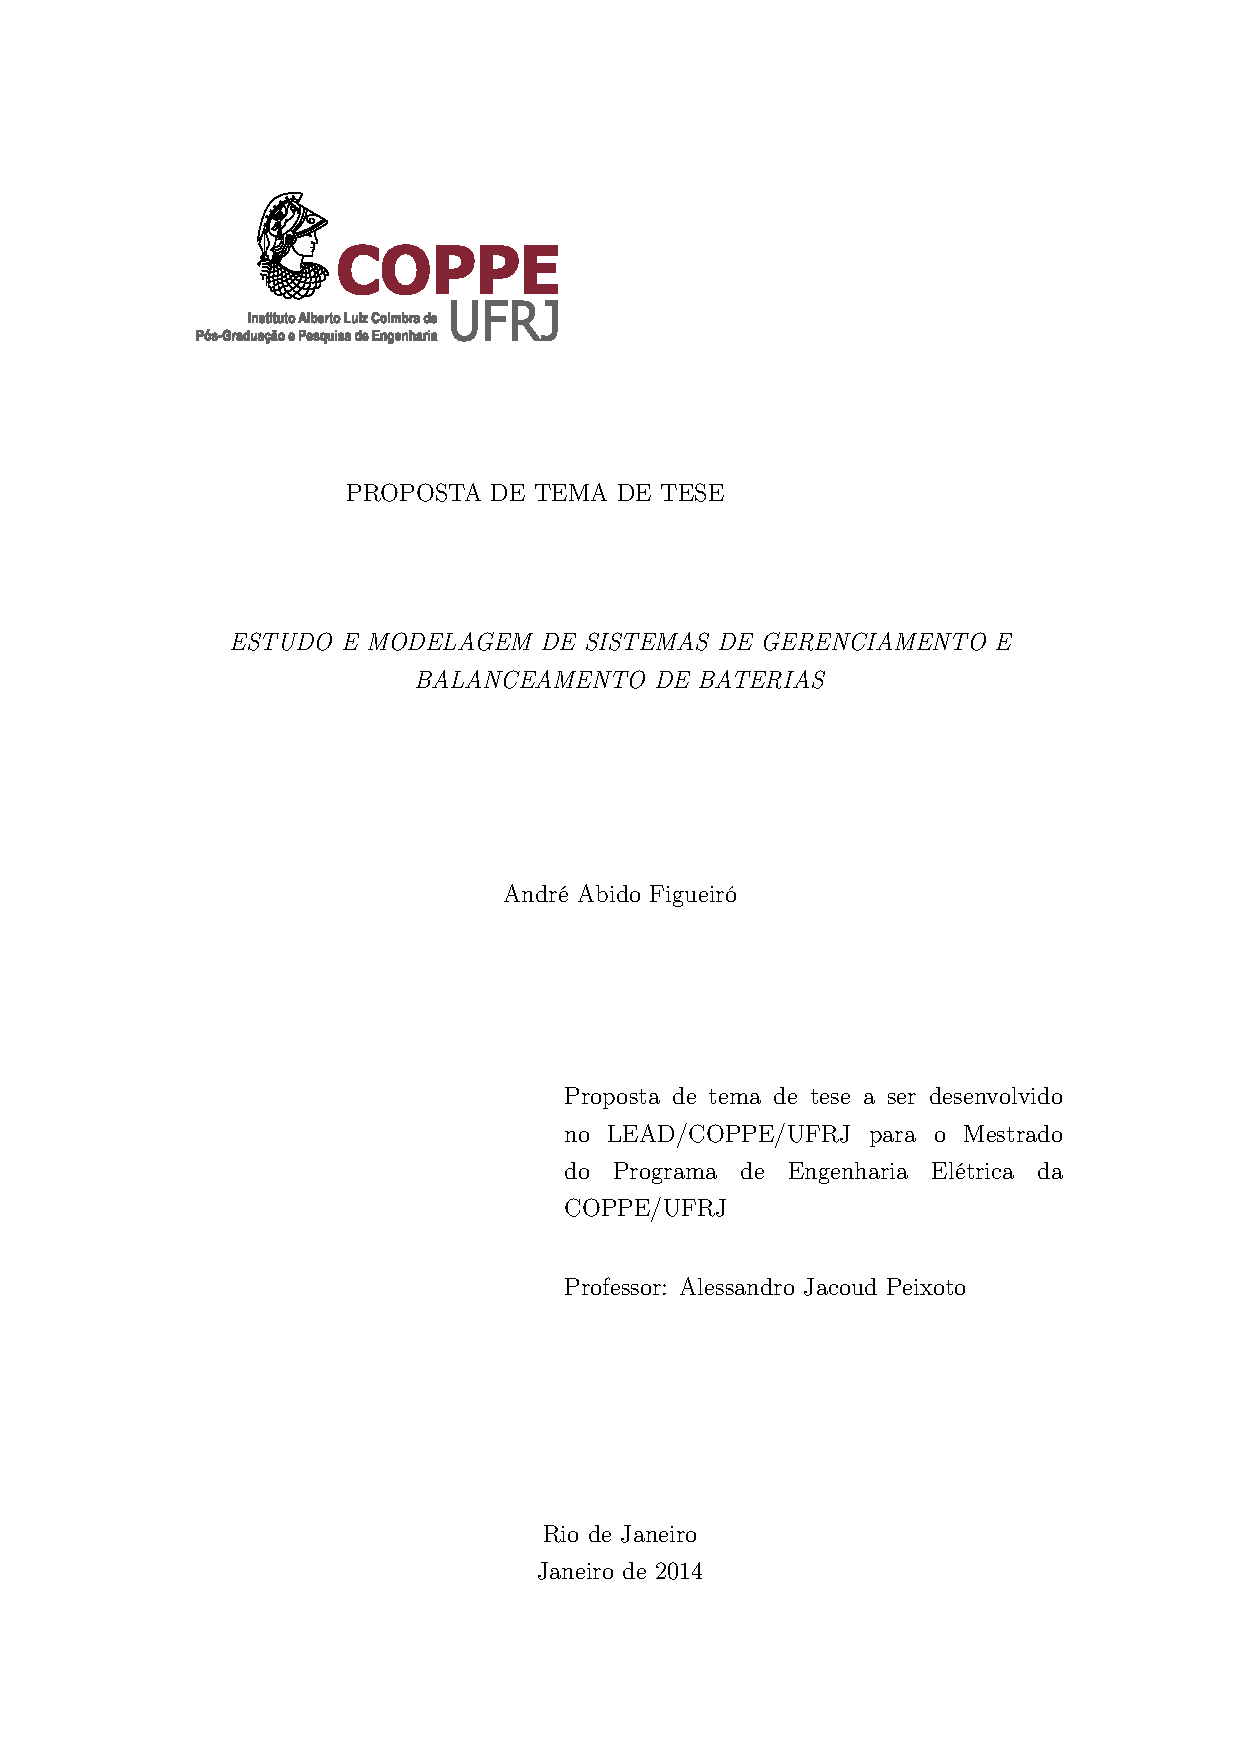
\includepdf[pages=-]{apendice-3-tese.pdf}

%--------------------------------------------------------------------- 

%\newpage%
%---------------------------------------------------------------------
%%% \section{Minutas}
%%%
%%% %---------------------------------------------------------------------
\subsubsection{Minuta de reuni�o (25-out-2013)}

\begin{tabbing}
  Local \= xxx \kill
  Local \> : LEAD \\
  Data  \> : 25 de Outubro de 2013 \\
  Hora  \> : 13:00
\end{tabbing}

%---------------------------------------------------------------------
\participantes{
  \jacoud,
  \andre,
  \elael,
  \julia,
  \patrick,
  \rafael,
  \ramon,
  \renan.
}

\begin{itemize}
  \item Update semanal. Resumo do que cada um estudou, as restri��es/recomenda��es e tarefas para a pr�xima semana.

  \begin{itemize}
    \item \textbf{\andre.} Estudou baterias e isolamento de cabos.
    Recomenda-se estudar sistemas de gerenciamento de pot�ncia e sincroniza��o dos equipamentos (time stamping).
    Pesquisar em ROV's: Sistemas de alimenta��o e umbilical. \\
    Nova Tarefa: Fazer um apanhado de possibilidades de sistemas de pot�ncia e umbilicais para saber qual se encaixaria melhor no projeto. \\

    \item \textbf{\rafael.} Novo bolsista de Mestrado. Tarefa preliminar: Explorar RockRobotics, familiarizar-se com a linguagem usada no projeto. \\
        Nova Tarefa: Instalar o ROCK, entender/familiarizar-se  com a programa��o do software e tentar resolver o primeiro exemplo do site. \\

    \item \textbf{\julia.} Trabalhando com identidade Visual, Planilha de aluguel Sylvain/ Invent�rio do Laborat�rio. \\
        Procedimentos de compras para o laborat�rio. \\
        Nova Tarefa: Site do projeto. Estrutura (perguntas, modelo, necessidades x usu�rios). Pesquisar sobre ROCK/Stoplogs, Pack Interface. \\
        Lembrete para Ramon: Contactar a acessoria de imprensa para divulgar o evento com a SBR em 3 de Nov. \\

    \item \textbf{\renan.} Foco em sensores de For�a. Fez pesquisa acessoria de forca, como os sensores funcionam, m�tricas importantes de mercado e o tipo de sensores que poder�amos usar no projeto. \\
        Nova Tarefa: Resumo de pros \& cons de sensores magn�ticos, focar em sensors a prova d'�gua.  Levantamento dos poss�veis m�todos para contato. Mini apresenta��o para ser discutida na semana que vem. \\

    \item \textbf{\elael.} Definido entre software e electr�nica, recomenda-se integra-lo no time de software que j� esta formado no LEAD. Estudou a documenta��o do ROCK.  \\
        Nova Tarefa: instalar o ROCK, entender/se familiarizar com a programa��o de software e tentar resolver o primeiro exemplo do site. Criar um drive. \\
  \end{itemize}

\end{itemize}

\vspace{10mm}%
\parbox[t]{70mm}{
  Aprovado por: \\[5mm]
  \centering
  %
\includegraphics[bb=1 1 1238 299,width=65mm]{../assinatura/assinatura-digital.jpg} \\[-4mm]
  
\includegraphics[width=65mm]{../assinatura/assinatura-digital.jpg} \\[-4mm]
  \rule[2mm]{70mm}{0.1mm} \\
  \ramon \\[1mm]
  Coordenador do Projeto \\
}

%---------------------------------------------------------------------
\fim


 \newpage%
%%% %---------------------------------------------------------------------
\subsubsection{Minuta de reuni�o (01-nov-2013)}

\begin{tabbing}
  Local \= xxx \kill
  Local \> : LEAD \\
  Data  \> : 01 de Novembro de 2013 \\
  Hora  \> : 13:00
\end{tabbing}

%---------------------------------------------------------------------
\participantes{
  \jacoud,
  \andre,
  \elael,
  \gabriel,
  \julia,
  \patrick,
  \rafael,
  \ramon,
  \renan.
}

\begin{itemize}
  \item Aprova��o da minuta.

  \item Discutir tarefas e recomenda��es da equipe para essa semana.

  \item Viagem a Porto Velho, Energia Sustent�vel do Brasil, adiada para o dia 10/11/2013.

  \item Update semanal. O que cada um do grupo desenvolveu durante a semana.
  \begin{itemize}
    \item \textbf{\andre.} N�o teve condi��o de pesquisar. Tarefa mantida para semana que vem. \\
        Tarefa: Pesquisa de possibilidades de sistemas de pot�ncia umbilical que se encaixem no projeto. \\

    \item \textbf{\rafael.} Cumpriu tarefa, instalou ROCK e fez o exerc�cio, familiarizando-se com a linguagem, criando drivers e library. \\

    \item \textbf{\julia.} Criative brief CIR. Atualizou planilhas de invent�rios e aluguel/ rockrobotics.org/ interface Package/reuni�o com professor Cl�udio Esperan�a/ Doris Kominsky. \\ Tarefas: criar o modelo do nosso site/ aulas de phyton/ computer logics (gradua��o) com Cl�udio Esperan�a. \\

    \item \textbf{\renan.} Apresentou pros \& cons de sensores magn�ticos e a prova d'�gua e fez um levantamento de poss�veis sensores e respectivos m�todos para contato. Garras atuadas. \\
        Tarefa: Sketch do equipamento inicial necess�rio, levantamento de sensor indutivo, camera guppy. Pesquisar a resist�ncia do a�o/underwater pump. \\

    \item \textbf{\elael.} Cumpriu tarefa. Encontrou alguns problemas de instala��o mas junto com o grupo de programa��o criou driver e explorou a linguagem. Tamb�m criou uma interface b�sica de controle usando Ruby. \\
        Tarefa: Tentar implementar sensors utilizados no ROCK. \\

    \item \textbf{\gabriel.} Cumpriu tarefa, encontrou alguns problemas de instala��o mas junto com o time de programa��o criou driver e explorou a linguagem. Quer relacionar o projeto com apresenta��o de aula de redes neurais. \\
        Tarefa: \\
  \end{itemize}

  \item Problemas em aberto:
  \begin{itemize}
    \item Procedimento de compras e medidas para as instala��es finais do laborat�rio.
    \item Op��es para a comprar de software, Adobe/ Solid Works/ Live Meeting/Bibliografia
    \item Fechar or�amento Invent�rio.
    \item Criar log para documentar problemas de ROCK/ criar um forum para colabora��o (?!)
    \item Dropbox para compartilhamento de arquivos.
    \item Viagem ESB/Relat�rio:
    \begin{itemize}
      \item Verificar encaixe (medi��o, propor��es) dos ganchos durante a visita a ESB para determinar que tipos de sensores podem ser implementados.
      \item Modelo detalhado do processo + Blueprints. \\
    \end{itemize}
  \end{itemize}

  \item Agenda para a pr�xima reuni�o:
  \begin{itemize}
    \item Resultado de pesquisas individuais.
    \item Relat�rio de viagem.
    \item Novas tarefas \& recomenda��es.
  \end{itemize}

\end{itemize}

\vspace{5mm}%
\parbox[t]{70mm}{
  Aprovado por: \\[5mm]
  \centering
  
\includegraphics[width=65mm]{../assinatura/assinatura-digital.jpg} \\[-4mm]
  \rule[2mm]{70mm}{0.1mm} \\
  \ramon \\[1mm]
  Coordenador do Projeto \\
}

%---------------------------------------------------------------------
\fim


 \newpage%

%---------------------------------------------------------------------
\fim

%---------------------------------------------------------------------
\end{document}
